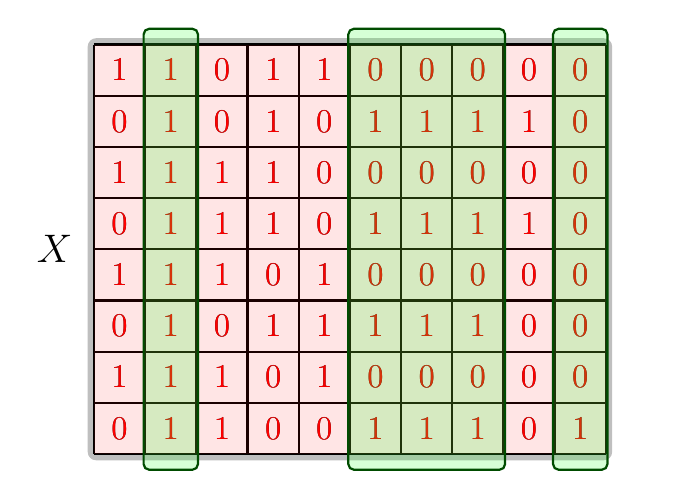
\begin{tikzpicture}
    \def\elements{{
            {1, 1, 0, 1, 1, 0, 0, 0, 0, 0},
            {0, 1, 0, 1, 0, 1, 1, 1, 1, 0},
            {1, 1, 1, 1, 0, 0, 0, 0, 0, 0},
            {0, 1, 1, 1, 0, 1, 1, 1, 1, 0},
            {1, 1, 1, 0, 1, 0, 0, 0, 0, 0},
            {0, 1, 0, 1, 1, 1, 1, 1, 0, 0},
            {1, 1, 1, 0, 1, 0, 0, 0, 0, 0},
            {0, 1, 1, 0, 0, 1, 1, 1, 0, 1}
        }}
    \def\result{{1, 0, 1, 1, 1, 1, 1, 0, 1}} 
    \def\n{9}
    \def\m{7}
    \def\step{0.65}

    \fill[gray!50, rounded corners = 3pt] (-0.08, 0.08) rectangle
        ({\step * (\n + 1) + 0.08}, {-\step * (\m + 1) - 0.08});
    \fill[white] (0, 0) rectangle ({\step * (\n + 1)}, {-\step * (\m + 1)}); 
    \draw[step = \step, thick] (0, 0) grid ({\step * (\n + 1)}, {-\step * (\m + 1)});

    \foreach \i in {0, 1, ..., \n}{
        \foreach \j in {0, 1, ..., \m}{
            \pgfmathparse{\elements[\j][\i]}
            \edef\val{\pgfmathresult}
            \ifthenelse{\val = 0}{
                \node at ({(\i + 0.5) * \step}, {-(\j + 0.5) * \step})
                    {\large \val};
            }{
                \node at ({(\i + 0.5) * \step}, {-(\j + 0.5) * \step})
                    {\textcolor{red}{\large \val}};
                \fill[red, opacity = 0.1]
                    ({\i * \step}, {-\j * \step})
                    rectangle
                    ({(\i + 1) * \step}, {-(\j + 1) * \step});
            }
        }
    }

    \uncover<2->{
        \draw[thick, green!30!black, rounded corners = 2pt, fill = green!80, fill opacity = 0.2]
            ({-0.02 + \step}, 0.2) rectangle ({\step * 2 + 0.02}, {-\step * (\m + 1) - 0.2});
    }

    \uncover<3->{
        \draw[thick, green!30!black, rounded corners = 2pt, fill = green!80, fill opacity = 0.2]
            ({-0.02 + \n * \step}, 0.2) rectangle
            ({(\n + 1) * \step + 0.02}, {-\step * (\m + 1) - 0.2});
    }

    \uncover<4->{
        \draw[thick, green!30!black, rounded corners = 2pt, fill = green!80, fill opacity = 0.2]
            ({-0.02 + 5 * \step}, 0.2) rectangle ({\step * 8 + 0.02}, {-\step * (\m + 1) - 0.2});
    }

 
    \node at (-0.5, {-\step * (\m + 1) / 2}) {\Large $X$};
    \node at ({\step * (\n + 1) + 0.5}, {-\step * (\m + 1) / 2}) {};

\end{tikzpicture}